% =====================================================================
%  Figure captions --- Attention-Allocated Retrieval
%
%  Every quantity quoted below is computed by
%  figures/generate_panels.py at draw time from validation/kernel/,
%  not transcribed from the results JSON. A caption and its panel
%  therefore cannot drift apart without the generator changing.
% =====================================================================

% ---------------------------------------------------------------------
%  PANEL 1
% ---------------------------------------------------------------------
\begin{figure*}[!htbp]
    \centering
    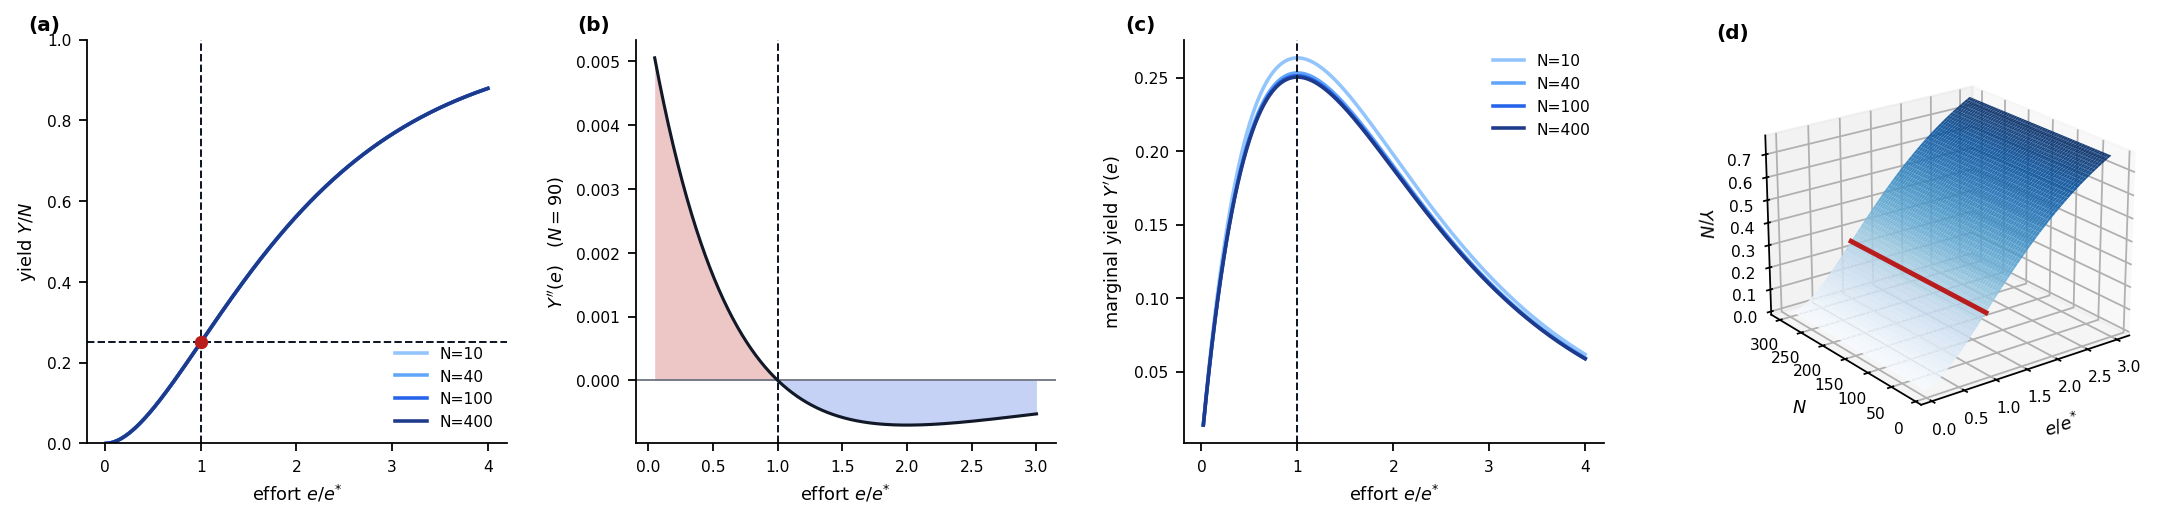
\includegraphics[width=\textwidth]{figures/panel_01_yield_surface.png}
    \caption{\textbf{The Federated-Join Yield Surface and Its Inflection.}
    (\textbf{A})~Normalised yield $Y(e)/N$ for corpus sizes $N \in \{10, 40, 100, 400\}$ against effort measured in units of each corpus's own threshold $e^{*}$. The four curves are drawn from $Y(e) = Np^2$ with $p = 1 - (1 - 1/N)^{e/2}$; because $p$ saturates and squaring a saturating function does not, every curve is sigmoid rather than concave. All four cross $Y/N = 0.25$ at exactly $e/e^{*} = 1$ (red marker), which is the quarter-corpus law: the yield at the inflection is $N/4$ for every $N$, with no asymptotics and no fitted constant.
    (\textbf{B})~Second derivative $Y''(e) = \tfrac{N}{2}(\ln q)^2 r(2r - 1)$, where $q = 1 - 1/N$ and $r = q^{e/2}$, evaluated at $N = 90$ ($e^{*} = 124.07$). The convex region $Y'' > 0$ is shaded red and the concave region $Y'' < 0$ blue. The sign change occurs at $e/e^{*} = 1$ and nowhere else, so the domain splits into exactly two branches: increasing returns below threshold, diminishing returns above it.
    (\textbf{C})~Marginal yield $Y'(e) = -Nrp\ln q$ for the same four corpora. Marginal yield does not decrease monotonically---it \emph{rises} to a peak at $e/e^{*} = 1$ before falling. This peak is the mechanism behind the necessary-versus-sufficient failure: at a budget just above $\sum_i e^{*}_i$ every source sits barely onto its concave branch where its marginal return is still near maximal, so withdrawing one source outright can free enough budget to push another further up its curve.
    (\textbf{D})~Yield surface $Y/N$ over $(e/e^{*},\,N)$ for $N \in [10, 300]$, with the threshold ridge $e = e^{*}(N)$ traced in red at constant height $0.25$. The ridge is flat in $N$: the inflection sits at the same normalised effort and the same fractional yield for every corpus size, which is why $e/e^{*}$ and not $e$ is the allocator's state variable.}
    \label{fig:panel1}
\end{figure*}

% ---------------------------------------------------------------------
%  PANEL 2
% ---------------------------------------------------------------------
\begin{figure*}[!htbp]
    \centering
    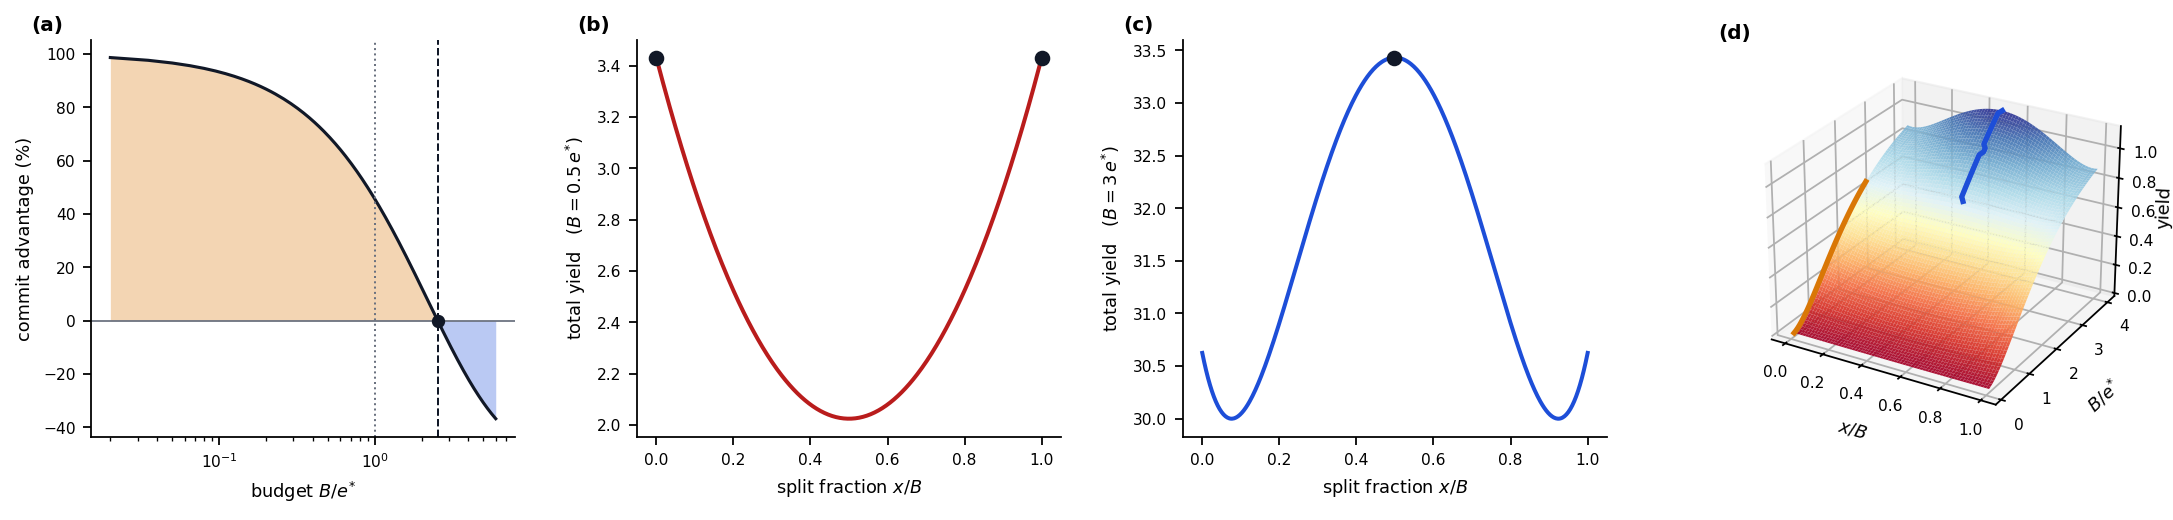
\includegraphics[width=\textwidth]{figures/panel_02_policy_reversal.png}
    \caption{\textbf{The Threshold Reverses Which Allocation Policy Is Optimal.}
    (\textbf{A})~Relative advantage of committing the whole budget to one source over splitting it evenly, against budget $B/e^{*}$ on a logarithmic axis, for two sources of equal corpus size $N = 40$. Committing wins by $98.6\%$ at $B = 0.02\,e^{*}$, by $45.7\%$ at $B = e^{*}$, and still by $12.5\%$ at $B = 2e^{*}$ where both sources are already on their concave branches. The advantage crosses zero at $u^{\dagger} = 2\log_2(1 + \sqrt{2}) = 2.5431$ (solid marker), \emph{not} at the dotted line $B = e^{*}$ where the yield curve inflects. The crossing is located by the plotting code rather than drawn at a predicted value, and the gap between $u^{\dagger}$ and the edge of the concave region at $u = 2$ is what falsified an earlier version of the reversal theorem.
    (\textbf{B})~Total yield against split fraction $x/B$ at a sub-threshold budget $B = 0.5\,e^{*}$. The curve is convex and attains its maximum at both endpoints ($3.431$ at $x/B \in \{0, 1\}$) against $2.025$ at the centre---a $69.4\%$ penalty for splitting. The optimum is \emph{at} a corner, not near one.
    (\textbf{C})~The same construction at a super-threshold budget $B = 3e^{*}$. The ordering has reversed: the maximum is the symmetric split ($33.43$ at $x/B = 0.499$) against $30.63$ at the endpoints. Water-filling is exactly right here and exactly wrong in (B).
    (\textbf{D})~Total yield over (split fraction, budget) for two equal corpora, with the ridge of optima traced---orange below the crossover, blue above. The ridge jumps from the boundary $x/B = 0$ to the centre $x/B = 1/2$ with no intermediate values, confirming the discontinuity: no asymmetric interior split is ever optimal, so an allocator cannot reach the answer by tuning a split fraction continuously.}
    \label{fig:panel2}
\end{figure*}

% ---------------------------------------------------------------------
%  PANEL 3
% ---------------------------------------------------------------------
\begin{figure*}[!htbp]
    \centering
    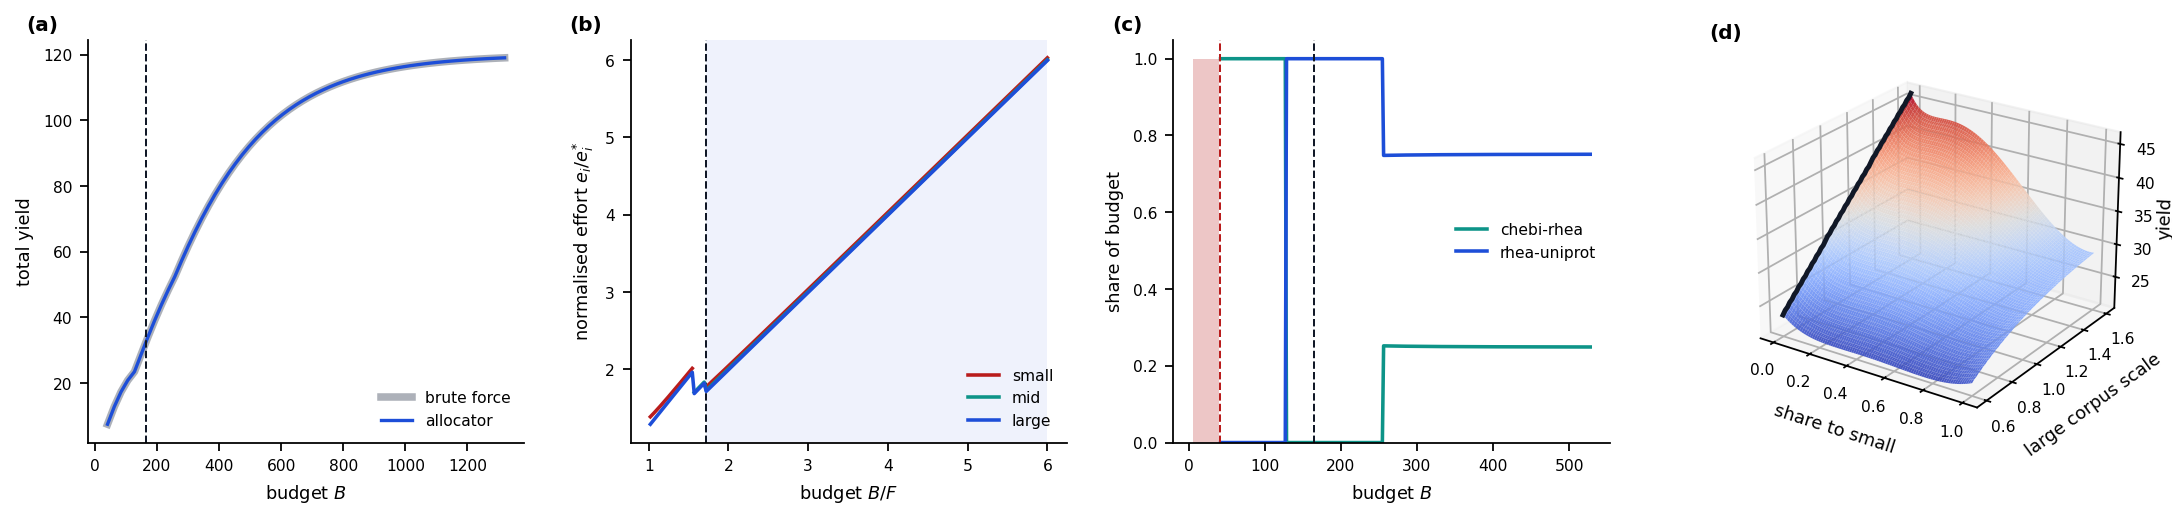
\includegraphics[width=\textwidth]{figures/panel_03_allocator.png}
    \caption{\textbf{The Gated Allocator Against Exhaustive Search.}
    (\textbf{A})~Allocator yield and brute-force yield against budget for the ChEBI--Rhea/Rhea--UniProt pair ($N = 30$ and $90$, so $e^{*}_1 = 40.89$, $e^{*}_2 = 124.07$, $F = \sum_i e^{*}_i = 164.96$). The two curves are visually indistinguishable across the full range; the worst relative gap over $60$ budgets is $9.3 \times 10^{-7}$, which is the resolution of the $800$-step brute-force grid rather than allocator error. The dashed line marks $B = F$.
    (\textbf{B})~Normalised efforts $e_i/e^{*}_i$ against budget $B/F$ for three unequal corpora $\{20, 60, 200\}$ ($e^{*} = 27.03,\,82.48,\,276.57$; $F = 386.07$). Within the shaded water-fill regime, which begins at $B/F = 1.72$, the three converge to a common value---at $B/F = 6$ they are $6.030$, $6.004$ and $5.996$, agreeing to $0.03$ despite raw efforts differing by an order of magnitude. To the left of the shaded band a source receiving nothing is drawn as a \emph{gap} rather than as zero, because there it is unfunded by design under the commit-subset rule and not an equalisation that failed.
    (\textbf{C})~Share of budget allocated to each source across the three policy regimes. Below $B = e^{*}_{\min} = 40.89$ (red dashed) the allocator refuses outright, shaded in red. Between $e^{*}_{\min}$ and roughly $1.7F$ it commits to a proper subset. Only above that does it water-fill, at which point both shares stabilise.
    (\textbf{D})~Total yield over (share to the small source, scale factor on the large corpus) at a budget just above $F$, with the argmax ridge traced in black. The ridge sits pinned at share $= 0$ across the whole range of corpus scalings: at $B = F$ exactly the marginal-equalising interior solution places both sources precisely at threshold and yields $N_1/4 + N_2/4 = 30$, while funding only the larger source yields $32.629$---$8.76\%$ more. Having every source on its concave branch is necessary for an interior optimum, not sufficient for it.}
    \label{fig:panel3}
\end{figure*}

% ---------------------------------------------------------------------
%  PANEL 4
% ---------------------------------------------------------------------
\begin{figure*}[!htbp]
    \centering
    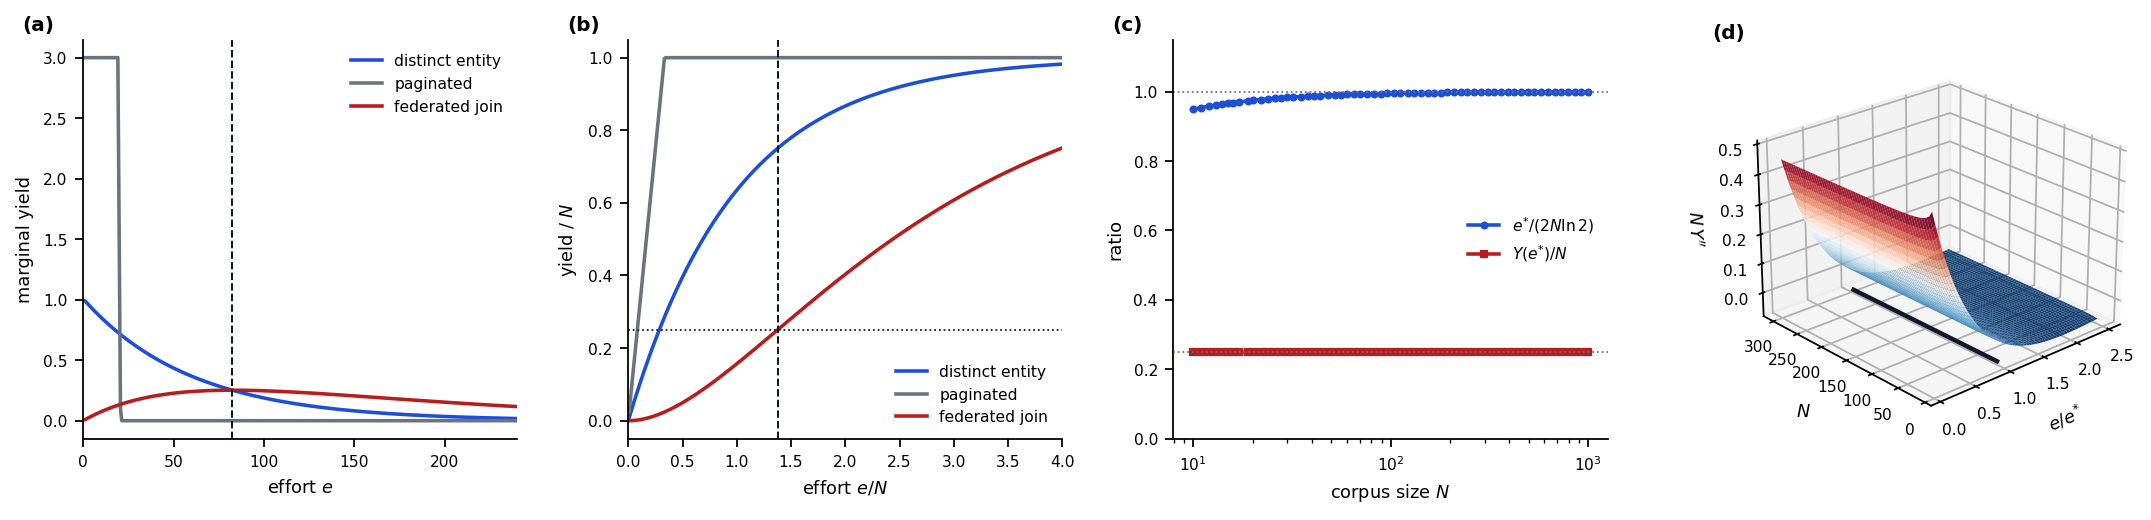
\includegraphics[width=\textwidth]{figures/panel_04_regimes.png}
    \caption{\textbf{Three Retrieval Regimes, and Two Constants Independent of Corpus Size.}
    (\textbf{A})~Marginal yield against effort for three retrieval regimes on common axes at $N = 60$ ($e^{*} = 82.48$, dashed). Distinct-entity retrieval follows coupon-collector coverage $N(1 - (1-1/N)^e)$ and falls monotonically. Paginated retrieval is flat at the page size until the corpus is exhausted, then zero. The federated join alone \emph{rises} to a peak at $e^{*}$ before falling. Only the join violates diminishing returns, and it does so across the entire sub-threshold range---so the assumption underpinning water-filling is environmental rather than structural, and it fails in precisely the environment a federated pipeline operates in.
    (\textbf{B})~The same three regimes as cumulative normalised yield $Y/N$ against $e/N$. The dotted line at $0.25$ and the dashed line at $e^{*}/N = 1.375$ intersect on the join curve, which is the quarter-corpus law located on the same axes as its two controls.
    (\textbf{C})~Two ratios against corpus size on a logarithmic axis, $N$ from $10$ to $10^{3}$. The asymptotic form of the threshold, $e^{*}/(2N\ln 2)$, approaches $1$ from below but is only $0.949$ at $N = 10$ and reaches $0.9995$ at $N = 1000$---an approximation that improves with $N$. The quarter-corpus law $Y(e^{*})/N$ is pinned at $0.25$ to within $3.0 \times 10^{-14}$ at every $N$ tested. One constant is asymptotic; the other is exact.
    (\textbf{D})~Scaled second derivative $N\,Y''$ over $(e/e^{*},\,N)$, red where convex and blue where concave, with the zero contour projected onto the floor. The contour is the plane $e = e^{*}$, flat in $N$: the boundary between increasing and diminishing returns sits at the same normalised effort for every corpus size, which is the threshold theorem rendered as a surface.}
    \label{fig:panel4}
\end{figure*}

% ---------------------------------------------------------------------
%  PANEL 5
% ---------------------------------------------------------------------
\begin{figure*}[!htbp]
    \centering
    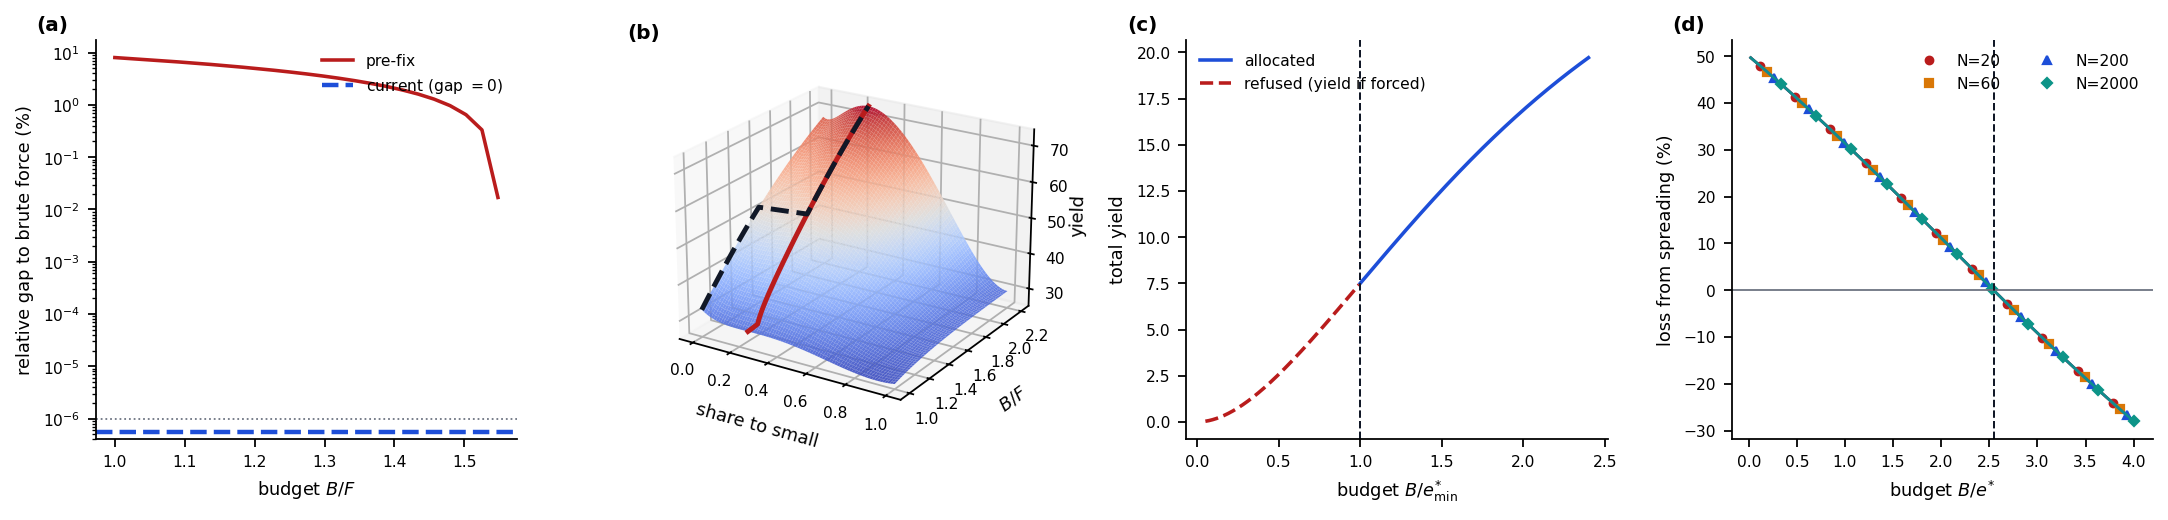
\includegraphics[width=\textwidth]{figures/panel_05_flaw_and_refusal.png}
    \caption{\textbf{An Allocator Flaw Caught by Brute Force, and the Refusal.}
    (\textbf{A})~Relative shortfall against exhaustive search, on a logarithmic axis, for the pre-fix allocation rule (water-fill whenever $B \geq F$) and for the shipped gated rule, over $220$ budgets from $F$ to $6F$. The pre-fix rule is suboptimal at $25$ of them, forfeiting up to $8.0566\%$ of the achievable yield at $B = F$ and recovering only past $B = 1.548F$. The gated allocator's shortfall is identically zero at every budget, so it has no curve to plot and is marked on the floor instead. A self-consistency check would have passed the broken rule; only comparison against a search sharing none of its reasoning exposed it.
    (\textbf{B})~The two allocations traced across the yield surface for $B/F \in [1.0, 2.2]$. The pre-fix interior solution (solid red) sits below the corner the gated rule selects (dashed black) precisely over the region where the surface is still convex, and the two merge once the budget is large enough that the interior solution is genuinely optimal.
    (\textbf{C})~Total yield against budget in units of $e^{*}_{\min} = 40.89$. Below $e^{*}_{\min}$ the allocator refuses to answer; the dashed red continuation is the yield it would have reported had it been forced to. The refusal is not a failure to compute---the number exists---but a statement that no allocation over these sources at this budget is defensible, computable from corpus size alone.
    (\textbf{D})~Loss from spreading rather than committing, against $B/e^{*}$, for four corpus sizes spanning two orders of magnitude ($N = 20, 60, 200, 2000$; markers offset along each curve so the overlap is visible). The four curves coincide to $1.3 \times 10^{-11}$ percentage points: in normalised effort $N$ cancels exactly, so the penalty for ignoring the gate is a function of $B/e^{*}$ alone. The loss runs from $49.7\%$ at $B = 0.02\,e^{*}$ through zero at $u^{\dagger} = 2.5431$ (dashed) to $-28.0\%$ at $B = 4e^{*}$, where spreading has become the better policy by the same margin.}
    \label{fig:panel5}
\end{figure*}
